In this chapter, we present \bpfcontain{}, an iteration on the original \bpfbox{} system
presented in \Cref{c:bpfbox}. \bpfcontain{} is a superset of \bpfbox. In particular, it is
a streamlined re-implementation that focuses on container-specific confinement policy, low
dependency overhead, and maximizing adoptability. Portions of this chapter are taken from
an upcoming paper, co-authored with David Barrera and Anil Somayaji, and planned for
submission at USENIX Security 2022. A draft of this paper is currently
available~\cite{findlay2021_bpfcontain}, although significant portions of this chapter
differ from the publicly available archive due to subsequent updates to \bpfcontain{}.



\section{\bpfbox{}'s Limitations and the Transition Toward \bpfcontain{}}%
\label{s:bpfcontain-bpfbox-limitations}

The previous chapter presented \bpfbox{}, a prototype process confinement mechanism and
precursor to \bpfcontain{}. While \bpfbox{} certainly offers a new perspective on
confinement and improves the status quo, the extent to which it achieves the design goals
outlined in \Cref{s:cp-design} of \Cref{c:confinement-problem} is arguably hampered by
a few inherent limitations. We enumerate and describe these limitations as follows.  The
goal is to examine these limitations as an early motivating factor for the development of
\bpfcontain{}, which will inform later comparisons between these two systems
(c.f.\ \Cref{s:bpfcontain-improvements}).

\begin{enumerate}
  \item \textbf{Dependency Overhead and Runtime Overhead.}
    Due to its userspace implementation using bcc, \bpfbox{} has a high dependency
    overhead. This overhead is the combined result of a number of requirements imposed on
    the host system by the bcc toolchain. On the userspace side, bcc depends on Python as
    well as the entire LLVM toolchain for program compilation. Both of these are rather
    hefty requirements on their own. Python requires an entire language runtime, and
    a full LLVM toolchain can introduce hundreds of megabytes of additional code
    (approximately 587MiB when installing LLVM version 12.0 on Arch Linux).

    Furthermore, Python and bcc incur significant runtime overhead. Python is an
    interpreted language with a much heavier runtime than compiled systems languages like
    C or Rust.  This runtime incurs additional performance disadvantages due to safety
    features like the global object lock, which impede concurrency. Since bcc compiles
    \gls{ebpf} programs at runtime, we incur additional compilation overhead for each
    program, sometimes resulting in significant startup delays depending on the complexity
    of the application. The runtime compilation of \gls{ebpf} programs also necessitates
    the availability of kernel headers as a compilation dependency in the target
    environment, adding further storage overhead (approximately 129MiB for Linux
    5.12 on a stock Arch kernel).

  \item \textbf{Lack of Container Semantics.}
    Although \bpfbox{} exposes a lightweight policy language with high-level semantics to
    the user, it fails to consider container semantics, as outlined in design goal
    \ref{i:dg-suitability} in \Cref{s:cp-design}. While this marks an improvement over
    existing confinement solutions by offering a terse yet expressive policy language, it
    fails to fully address the container-specific use case; in other words, \bpfbox{} is
    more suitable to generic, ad-hoc application sandboxing than to container-specific
    applications. In improving how the \bpfbox{} model handles containers, we can
    simultaneously simplify policies and improve security by defining a clear protection
    boundary around a container.

  \item \textbf{Policy Language Improvements.}
    In addition to adding container semantics, other aspects of the \bpfbox{} policy
    language can also be improved and simplified. For instance, \bpfbox{} implements
    policy in a domain-specific policy language, designed specifically with \bpfbox{}'s
    enforcement engine in mind. While effective, this approach is tightly-coupled with
    policy enforcement and introduces additional cognitive overhead when making extensions
    to or modifying the policy language design. Furthermore, learning the syntax of
    a custom policy language can introduce an additional barrier-to-entry for new policy
    authors, to the detriment of \bpfbox{}'s original goal of making policy authorship
    available to end users.
\end{enumerate}

\subsection{Motivating \bpfcontain{}}

The key insight behind \bpfcontain{} is that \bpfbox{} approached the confinement problem
(c.f.\ \Cref{c:confinement-problem}) from a \textit{per-process} perspective. When dealing
with containers, we should instead approach the confinement problem from
a \textit{per-process-group} perspective. That is, we expand the unit of confinement from
an individual process to a collection of related processes. Specifically, our goal is to
define a clear boundary between the container and the outside world, while minimizing the
friction between two subjects that operate within this boundary.

Under \bpfbox{}, policies applied to individual applications, inheriting policy across
forks, and selectively transitioning across execves. While this model is effective for
application-level confinement, it fails to meet the needs of a container-specific
deployment.  Conversely, \bpfcontain{} expands this model to incorporate container
semantics, grouping processes into a container and enforcing a protection boundary around
the container.  Implementing confinement in this way requires some fundamental changes to
both the underlying policy language and policy enforcement mechanism. In particular, we
alter the policy language to work with higher level semantics that support container-level
confinement. Moreover, \bpfcontain{}'s enforcement engine employs a more nuanced default
policy that considers the relationship between processes and resources that exist within
the context of a container. These changes from a policy and enforcement perspective enable
\bpfcontain{} to enforce simple container-level policies while reusing the initial ideas
from \bpfbox{}: namely, dynamic, lightweight enforcement based on \gls{ebpf}.

While implementing \bpfcontain{}, opportunities arose to improve how it handles
dependencies and manages the lifecycle of its \gls{bpf} programs and maps. Specifically,
we architect \bpfcontain{} based on Rust, libbpf-rs~\cite{libbpf-rs}, and \gls{bpf}
\gls{core}~\cite{nakryiko2020_core}. These changes totally eliminate the runtime overhead
introduced by \gls{bpf} program compilation and the dependency overhead from LLVM and
kernel headers. Further, \gls{core} enables \bpfcontain{} to work seamlessly across
multiple kernel versions and configurations. These changes improve the adoptability of
\bpfcontain{}, particularly in containerized environments, wherein heavyweight
dependencies can critically impact deployments.

\Cref{tab:bpfcontain-comparison} offers a high-level comparison between the properties and
features of \bpfbox{} and \bpfcontain{}. This comparison provides a high-level overview of
the major differences and motivating properties in each design. The sections that follow
will discuss each of these items in detail.

\begingroup\small
\begin{longtable}[c]{r||ll}
\caption[Comparing \bpfbox{} and \bpfcontain{}]{
    Comparing \bpfbox{} and \bpfcontain{} by their properties and how well each satisfies
    the design goals outlined in \Cref{s:cp-design}.
}%
\label{tab:bpfcontain-comparison}\\
  \toprule
  Property/Goal              & \bpfbox{}        & \bpfcontain{} \\
  \midrule
  Userspace Implementation   & Python + bcc     & Rust + libbpf-rs\\
  Kernelspace Implementation & bcc + LLVM       & \glsentryshort{bpf} \glsentryshort{core} \\
  Dependencies               & $>800\text{MiB}$ & $<5\text{MiB}$ \\
  State Management           & Process-Level    & Container-Level    \\
  Default Policy             & Default-Deny     & Container Boundary\textsuperscript{\textdagger} \\
  Policy Language            & Custom DSL       & YAML/JSON/TOML \\
  \midrule
  Simple/Flexible Policies?  & Yes              & Yes \\
  Suitable for Containers?   & No               & Yes \\
  High Adoptability?         & Somewhat\textsuperscript{\textdaggerdbl}         & Yes \\
  \bottomrule
  \multicolumn{3}{p{4.5in}}{\footnotesize \textsuperscript{\textdagger}\bpfcontain{}'s policy
  defaults are more nuanced than \bpfbox{}. We enforce a default-allow policy on resources
  \textit{within} the container, and a default-deny policy on resources \textit{outside}
  of the container. See \Cref{ss:bpfcontain-default} for details.}\\
  \multicolumn{3}{p{4.5in}}{\footnotesize \textsuperscript{\textdaggerdbl}While \bpfbox{} has
  a more adoptability than an out-of-tree \gls{lsm} (due to \gls{ebpf}), its practical
  adoption is hampered by heavy runtime dependencies and incompatibility with the
  container model.}
\end{longtable}
\endgroup

\section{\bpfcontain{} Overview}%
\label{s:bpfcontain-overview}

\bpfcontain{} is a container security daemon for Linux with an emphasis on simple,
high-level confinement policies for container deployments. Although it is expressly
designed to work with container semantics in mind, \bpfcontain{} implements a superset of
\bpfbox{}'s capabilities (c.f.\ \Cref{c:bpfbox}) and works for confining ordinary
applications as well as containers. To achieve confinement, \bpfcontain{} leverages
\gls{ebpf} programs attached to \gls{lsm} hooks in the kernel for security enforcement.

As a container-specific confinement solution, \bpfcontain{} has a number of important
design goals, some of which are shared with \bpfbox{}. First, we seek to design a simple
yet flexible policy language that supports ad-hoc confinement use cases, enabling an
end user to write a custom confinement policy to suit their needs. We extend this goal by
seeking to make the policy language and enforcement engine \textit{container specific}.
This means that \bpfcontain{} policies should conform to container semantics and work in
tandem with container virtualization primitives to improve policy enforcement and further
simplify the underlying policies. An implicit sub-goal of container-specific policy is to
improve the level of confinement afforded to container deployments, bringing security more
in line with that of alternative isolation techniques, such as virtual machines. Finally,
\bpfcontain{} should be readily adoptable in production use cases and should be useful for
confining existing container workloads.

At the surface level, \bpfcontain{}'s architecture is similar to that of \bpfbox{}, albeit
with significant differences in implementation and design details. In a nutshell,
\bpfcontain{} is implemented as a privileged userspace daemon that loads \gls{ebpf}
programs and maps into the kernel, which then enforce policy.
\Cref{ss:bpfcontain-enforcement-overview} provides a high-level overview of how
\bpfcontain{} enforces policy, whereas \Cref{s:bpfcontain-implementation} covers
\bpfcontain{}'s architecture and implementation details in full.

\subsection{Policy Enforcement at a High Level}%
\label{ss:bpfcontain-enforcement-overview}

\bpfcontain{} enforces confinement policy using \gls{ebpf} programs attached to \gls{lsm}
hooks in the kernel. Like \bpfbox{}, \bpfcontain{} leverages the
\gls{krsi}~\cite{singh2019_krsi} \gls{lsm} programs introduced in Linux 5.7 for this
purpose. Unlike \bpfbox{}, \bpfcontain{} generates \gls{bpf} bytecode at
\textit{compile time} rather than at runtime. The bytecode is then embedded directly in
\bpfcontain{}'s binary object file, where it can subsequently be loaded into the kernel at
runtime. This has the benefit of eliminating initial compile-time overhead and supporting
cross-architecture deployments using \gls{bpf} \gls{core}.

To confine a container, an administrator authors a high-level confinement policy that
specifies which operating system interfaces and resources should be exposed to the
container.  Thanks to a modular approach to encoding and decoding policies, \bpfcontain{}
policies may be written in a number of user-facing data serialization languages, including
YAML~\cite{yaml}, TOML~\cite{toml}, and JSON~\cite{json}. (For the rest of this thesis, we
assume the YAML format for simplicity.) At a minimum, \bpfcontain{} policies include
a policy name, along with a few tunable parameters. From there, the administrator may
specify zero or more policy rules over three distinct categories: allow, deny, and taint.
We cover \bpfcontain{} policy in more detail in \Cref{s:bpfcontain-policy}.

\begin{figure}[htpb]
  \centering
  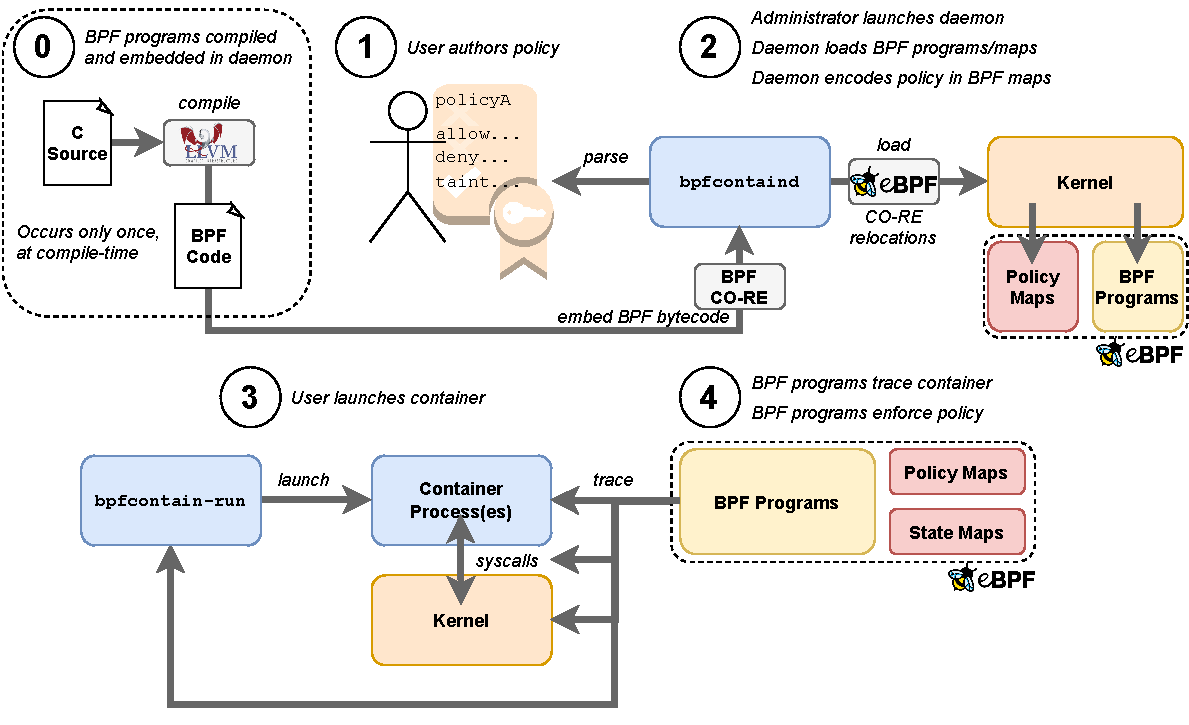
\includegraphics[width=1\linewidth]{figs/bpfcontain/overview.pdf}
  \caption[A high-level overview of how \bpfcontain{} confines containers]{
    A high-level overview of how \bpfcontain{} confines containers.  At compile-time,
    the object code for \bpfcontain{}'s \gls{bpf} programs is embedded directly into the
    resulting binary. To confine a container, the user first authors a high-level policy
    in their chosen data serialization language. The daemon parses this policy and loads
    it into the kernel by encoding it into \gls{ebpf} maps. The user then launches the
    container using the \texttt{bpfcontain-run} wrapper, at which point \bpfcontain{}
    begins tracing it and enforcing policy. Note the subtle differences between this
    figure and \Cref{fig:bpfbox-policy-overview} in \Cref{c:bpfbox}.
  }%
  \label{fig:bpfcontain-overview}
\end{figure}

The \bpfcontain{} daemon runs as a privileged process, parsing and loading user policy by
encoding it into a series of \gls{bpf} maps. The user then launches their container using
an unprivileged wrapper program, \texttt{bpfcontain-run}. The sole task of this wrapper
application is to invoke a stub function which does nothing more than pass the desired
policy ID as an argument. \bpfcontain{} traces this function call and uses it to confine
the container with the correct policy. Unlike \bpfbox{}, this technique enables the user
to associate any container with any policy, rather than a fixed one-to-one mapping.

At runtime, \bpfcontain{}'s \gls{bpf} programs trace the behaviour of processes running
under the container and confine it according to a mixture of default policy and policy
rules specified by the user. Like \bpfbox{}, enforcement is accomplished primarily through
\gls{bpf} programs attached to \gls{lsm} hooks in the kernel. The precise implementation
details of these programs vary significantly, and are covered in detail in
\Cref{s:bpfcontain-implementation}. \Cref{fig:bpfcontain-overview} illustrates
a high-level overview of the policy enforcement process described here.



\section{\bpfcontain{} Implementation}%
\label{s:bpfcontain-implementation}

This section presents the implementation details and architecture of \bpfcontain{}'s
policy enforcement mechanism. Specifically, we provide an initial overview of
\bpfcontain{}'s userspace and kernelspace components, then examine how \bpfcontain{}
enforces policy in the kernel using \gls{ebpf}. Whereas this section focuses specifically
on policy enforcement, \Cref{s:bpfcontain-policy} outlines and documents the details of
\bpfcontain{}'s policy language.

\subsection{Architectural Overview}%
\label{ss:bpfcontain-architecture}

Like \bpfbox{}, \bpfcontain{} is implemented as privileged daemon that runs in userspace
and loads \gls{ebpf} code into the kernel for policy enforcement. However, the precise
architecture and implementation details of this daemon are quite different. In particular,
the daemon is implemented in Rust and leverages the libbpf-rs crate\footnote{A crate is
a Rust package that can be added as a dependency to a project. For the purposes of this
thesis, we can consider the terms \enquote{crate} and \enquote{library} to be
equivalent.}~\cite{libbpf-rs} to load its \gls{ebpf} programs and maps into the kernel.
This results in a number of advantages, which we discuss in more detail in the following
section.

\bpfcontain{}'s kernelspace \gls{ebpf} programs trace container lifecycle and enforce
policy, while \gls{ebpf} maps store policy and pass intermediary state between program
invocations. This architecture is similar in spirit to the design of \bpfbox{}, but with
a few fundamental differences. Rather than using the LLVM toolchain to compile
programs at runtime, \bpfcontain{} pre-compiles and embeds the \gls{bpf} object code into
its binary object file. Using \gls{bpf} \gls{core}~\cite{nakryiko2020_core}, these
programs can then be dynamically loaded into any supported kernel, regardless of the
underlying configuration or architectural details.

\bpfcontain{} leverages several \gls{bpf} program and map types to implement container
tracing and confinement. While many of the major program types are shared with \bpfbox{},
there are a few distinct differences (c.f.\ \Cref{ss:bpfbox-architecture}). We enumerate
these differences as follows. Map types are outlined in \textbf{\green{green}} and program
types are outlined in \textbf{\purple{purple}}.

\paragraph*{Maps:}
\begin{itemize}
  \item \bpfcontain{} replaces many of \bpfbox{}'s \textbf{\green{Hash Maps}},
  particularly those used to track process state, with equivalent \textbf{\green{Local
  Storage Maps}}. Local storage is a new \gls{ebpf} map type supported in the latest
  kernels (Linux 5.11 and onwards). Local storage maps tether the underlying value to
  a kernel data structure, such as a task or inode, used as a key into the map. The result
  is a dynamically-allocated and garbage-collected per-structure storage blob.
  \bpfcontain{} leverages these for more memory-efficient storage of per-task and
  per-inode state.
\end{itemize}

\paragraph*{Programs:}
\begin{itemize}
  \item \bpfcontain{} replaces the use of scheduler \textbf{\purple{Tracepoints}} with
  equivalent \textbf{\purple{\gls{lsm} Probes}} that expose the same information. This
  reduces potential overhead from multiple \gls{bpf} program invocations on the same code
  path, most notably over \texttt{fork(2)} and \texttt{clone(2)} family system calls.

  \item \bpfcontain{} uses \textbf{\purple{Fentry and Fexit}} probes in place of
  \textbf{\purple{Kprobes}}. These use a more efficient trampoline technique for program
  entry and use \gls{btf} information exposed by the kernel for direct memory access,
  making them far more efficient than kprobes\footnote{However, the majority of \bpfbox{} and
  \bpfcontain{}'s \gls{ebpf} programs are \gls{lsm} probes rather than kprobes or fentry
  probes. As a result, this design change has little consequence on overall performance overhead.}.
\end{itemize}

Aside from the aforementioned differences, \bpfcontain{} uses the same \gls{bpf} program
and map types as \bpfbox{}. However, the underlying implementation details of each
\gls{bpf} program will be quite different from \bpfbox{}, as \bpfcontain{} is dealing with
container semantics, new policy rules, and more nuanced policy defaults. We examine the
most important implementation details in the subsections that follow.



\subsection{Policy Deserialization and Loading}%
\label{ss:bpfcontain-serde}

When designing the \bpfcontain{} policy language, we made a conscious design decision to
avoid constraining the user to one specific language syntax. In particular, we wanted to
avoid another domain-specific language, as learning the policy language could be a barrier
to entry for new users. A domain-specific policy language also presents issues when making
changes to or adding new features to the policy language specification, as the parser and
lexer must both be modified, along with underlying rule representation and enforcement
engine. Instead, we elected to decouple the policy language from the policy specification,
using Serde~\cite{serde}, a data serialization and deserialization crate for Rust.

Serde leverages Rust's powerful type system and procedural macros to derive serialization
and deserialization logic for vanilla Rust structs and enums. Rust crates that consume
Serde's \gls{api} can then use the automatically generated logic for serialization and
deserialization. This design enables a plug-and-play relationship between a data schema,
defined as a Rust data structure, and any data serialization language supported through the
Rust crates ecosystem. \bpfcontain{} uses Serde to automatically generate the accompanying
deserialization logic for a \texttt{Policy} struct and several \texttt{Rule} structs, one
for each supported rule type. \Cref{lst:bpfcontain-serde} depicts a simplified example of
how this works.

\begin{lstlisting}[language=Rust, gobble=2, caption={[A simplified example of \bpfcontain{}'s policy deserialization logic]
  A simplified example of \bpfcontain{}'s policy deserialization logic. Policy rules are
  specified declaratively using Rust structs and the corresponding deserialization logic
  is automatically generated by the Serde crate using a simple decorator macro.
},
label={lst:bpfcontain-serde}]
  use serde::Deserialize;

  /// The policy data structure
  #[derive(Deserialize)]
  pub struct Policy {
    name: String,
    /* Other policy metadata would go here... */
    allow: Vec<Rule>,
    deny: Vec<Rule>,
    taint: Vec<Rule>,
  }

  /// An enum encompassing all rule types
  #[derive(Deserialize)]
  pub enum Rule {
    FileRule(FileRule),
    /* Other rule types would go here... */
  }

  /// A "file access" rule
  #[derive(Deserialize)]
  pub struct FileRule {
    pathname: String,
    access: String,
  }

  /* Other rule types would go here... */
\end{lstlisting}

To enable the daemon to encode policy as an \gls{ebpf} map, each rule type implements the
\texttt{LoadableRule} trait. The daemon uses this logic to convert a policy rule into
a canonical format that can be represented in the kernel and thus used to enforce security
policy. Implementing this trait is as simple as writing a \texttt{load()} function that
makes a series of map updates to load the rule into the kernel; we leverage
libbpf-rs~\cite{libbpf-rs} for this purpose. When loading a policy into the kernel, the
daemon simply invokes this \texttt{load()} function for each policy rule.

Implementing policy deserialization and loading logic in this way has a number of
advantages. Since the policy schema is simply encoded declaratively in vanilla Rust, it is
easy for a developer (even a new contributor to \bpfcontain{}) to implement a new rule
type and add it to \bpfcontain{}. Adding a new rule type is as simple as defining a new
Rust data type to represent the rule and implementing the \texttt{LoadableRule} trait,
enabling the daemon to encode the rule as an \gls{ebpf} map. Due to Serde's modular
design, supporting a new serialization language for \bpfcontain{} policies is trivial; we
simply pull in the corresponding consuming crate as a dependency. Currently, \bpfcontain{}
supports YAML, JSON, and TOML as policy language encodings, but this can easily be
extended in future versions.

While these conveniences may add some modest performance overhead, this overhead is
incurred at policy load time and has no impact on any of \bpfcontain{}'s kernelspace code
paths. Therefore, we expect the overall impact of this design choice on system
performance to be minimal.

\subsection{Policy Enforcement}%
\label{ss:bpfcontain-enforcement}

Policy enforcement under \bpfcontain{} can be thought of as a combination of
\textit{explicit policy} (the rules defined in the policy file) and a nuanced
\textit{default policy} (the set of sensible defaults that \bpfcontain{} enforces to
define a boundary around the container). In particular, default access to resources is
determined based on whether that resource exists within the context of a container.
Resources within the container, such as \gls{ipc} handles into container processes or
filesystems belonging to the container's user namespace mount are considered
default allow. Conversely, resources outside of the container, such as external files or
processes, are considered default deny. Similarly, access is also denied to any operating
system interfaces that could affect global system state, such as character devices, kernel
modules, \gls{ebpf}, and some special filesystems. Exceptions to these defaults may
be explicitly defined in the policy file as required. \bpfcontain{} currently uses
ad-hoc information gathered at runtime to enforce its default policy; future integration
with container runtimes (discussed in \Cref{s:disc-future-work}) could significantly
improve container-specific policy defaults in the future. \Cref{ss:bpfcontain-default}
examines the implementation of \bpfcontain{}'s default policy in more detail.

Like \bpfbox{}, \bpfcontain{} maintains its policy files in a root-controlled directory
(\texttt{/var/lib/bpfcontain/policy} by default). These policy files may be written in any
policy language supported by \bpfcontain{}'s policy deserializer, as documented in
\Cref{ss:bpfcontain-serde}. The \bpfcontain{} daemon watches the policy directory for
updates to policy files and triggers a reload of the corresponding policy when a file
changes. To load a policy, the daemon deserializes the policy file into a Rust data
structure consisting of a series of policy rules and accompanying metadata. It then
encodes this policy structure into a series of resource IDs and access vectors and loads
these into the correct policy maps in the kernel using the \texttt{bpf(2)} system call.
Once a policy has been loaded into the kernel, \bpfcontain{}'s \gls{ebpf} programs can
begin enforcing it.

To start confinement, a user invokes an unprivileged application, \texttt{bpfcontain-run},
which wraps the target executable. This wrapper's only purpose is to enable
\bpfcontain{}'s \gls{ebpf} programs to associate its process group with the correct policy
in the kernel.  This is done by invoking a stub function, traced by a \gls{usdt} probe.
When the probe fires, it reads the policy ID, passed as an argument to the stub, along
with other information such as the task's \gls{pid} and namespace membership taken from
its task struct in the kernel. The probe then updates a global process state map with this
information. Subsequent \gls{ebpf} programs use this information when making enforcement
decisions and when managing the container's state. \Cref{ss:bpfcontain-state} describes
state management in more detail.

\bpfcontain{} enforces most policy rules using \gls{krsi}~\cite{singh2019_krsi}, which
enables it to attach \gls{ebpf} programs to \gls{lsm} hooks in the kernel. In cases where
\gls{lsm} hooks alone are insufficient or no \gls{lsm} hook is exposed to guard the target
operation, \bpfcontain{} falls back to an fentry probe, hooking the underlying kernel
functions directly. In total, \bpfcontain{} instruments 46 \gls{lsm} probes, covering
filesystem, network socket, \gls{ipc}, and capability-level access, in addition to
miscellaneous privileged operations like loading a kernel module or updating an \gls{ebpf}
program or map. One fentry probe is used to prevent a container from modifying its
namespace membership after starting confinement.

\bpfcontain{} supports four distinct policy decisions for security-sensitive operations:
\texttt{allow}, \texttt{deny}, \texttt{taint}, or \texttt{forcequit}. A decision of
\texttt{allow} causes the access to be allowed, as normal. A decision of \texttt{deny}
results in the access being denied, and the corresponding system call returning
\texttt{-EACCES} to the user. A decision of \texttt{taint} causes \bpfcontain{} to taint
the container, a process that is similar in spirit to tainting under \bpfbox{}
(c.f.\ \Cref{ss:bpfbox-enforcement} of \Cref{c:bpfbox}). When a container is tainted, it
transitions into a stricter default-deny policy. Finally, a decision of \texttt{forcequit}
causes the kernel to terminate the offending process by delivering an uncatchable
\texttt{SIGKILL}\footnote{\texttt{SIGKILL} is a POSIX signal that causes a process to
immediately force quit. Unlike most signals, this signal cannot be ignored or handled by
the process.}. This decision is reserved for aggressive violations of \bpfcontain{}'s
default policy, such as a process attempting to load code into the kernel
(c.f.\ \Cref{ss:bpfcontain-default}).

When enforcing policy, \bpfcontain{} employs a simple heuristic to judge what the
resulting policy decision should be. If any rule matches a \texttt{deny} decision, the
operation is denied. If any rule matches a \texttt{taint} decision, the container is
tainted.  Finally, if no rule matches a \texttt{deny} decision and any rule matches an
\texttt{allow} decision, the operation is allowed. In the case where no rule matches are
found, \bpfcontain{} falls through to its default policy (\Cref{ss:bpfcontain-default}).
This process is depicted in full in \Cref{fig:bpfcontain-enforcement} on page
\pageref{fig:bpfcontain-enforcement}.

\subsection{Default Policy}%
\label{ss:bpfcontain-default}

Since \bpfcontain{} is designed to confine containers, it is able to achieve some nuanced
policy defaults by leveraging container-level semantics. This marks a significant
improvement over both conventional \glspl{lsm} such as SELinux and AppArmor, and the
original \bpfbox{} system, which each require the user to either explicitly mark each
desired access or to over-generalize access in favour of simpler policies. By taking
container semantics into account, \bpfcontain{} policies can be simultaneously expressive
and secure yet offer a simple path to achieving strong protection defaults.
\Cref{fig:bpfcontain-enforcement} depicts \bpfcontain{}'s default enforcement strategy.

\begin{figure}[p]
  \centering
  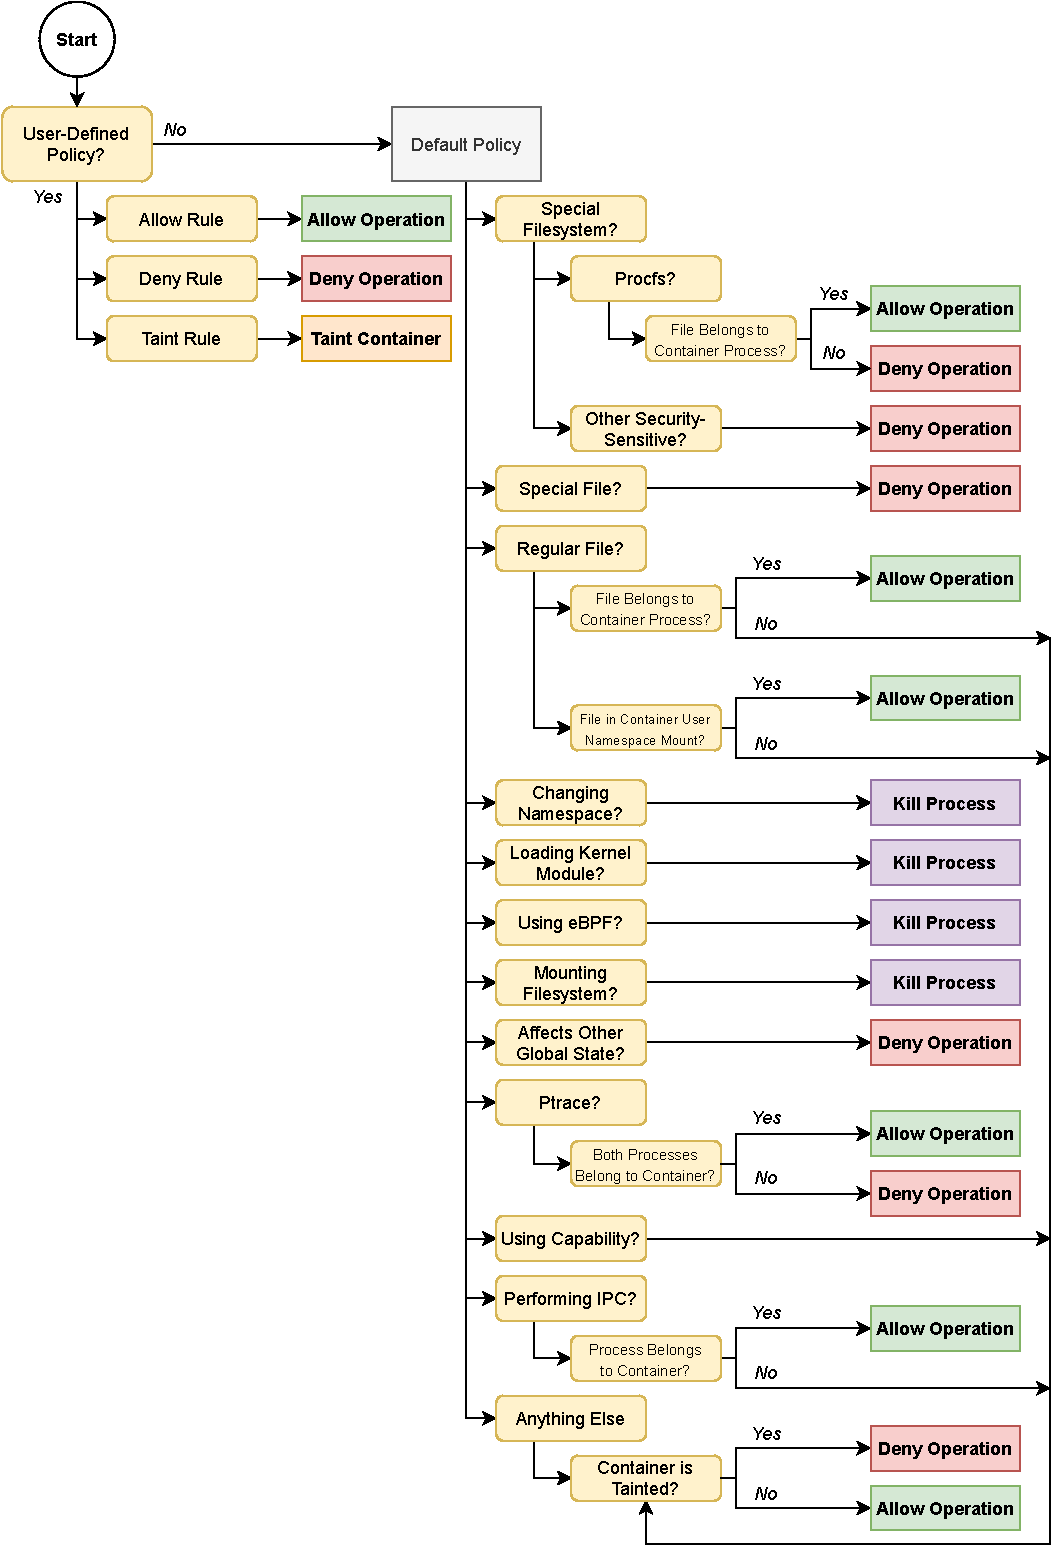
\includegraphics[width=0.75\linewidth]{figs/bpfcontain/enforcement.pdf}
  \caption[The policy enforcement strategy under \bpfcontain{}]{
    The policy enforcement strategy under \bpfcontain{}, expressed as a flowchart. Using
    container semantics, \bpfcontain{} achieves rich policy defaults, denying access to
    global resources and operations which can affect global system state while preserving
    intra-container access. This greatly simplifies the resulting confinement policy and
    enables the user to focus on specific exceptions to default protection.
  }%
  \label{fig:bpfcontain-enforcement}
\end{figure}

\bpfcontain{}'s default policy depends largely on the type of access that a container is
requesting. If the requested access is to a regular file, \bpfcontain{} checks to see if
this file exists under the container's user namespace, provided that this namespace is
non-global. This covers, for example, a temporary or overlay filesystem mounted within
a non-global user namespace.  Similarly, default \gls{ipc} access is gated by whether or
not the processes on either end of the \gls{ipc} handle belong to the same container. If
they do, access is granted; otherwise, access is denied. Ptrace is similarly restricted;
a process may only ptrace another if both processes exist in the same container. In this
way, we preserve the semantics of the container: resources that exist \textit{within}
a container are accessible by processes within the same container, but resources
that exist \textit{without} are not be accessible by default.

Special files such as character or block devices are treated separately from regular
files. Since these provide direct interfaces into the kernel, it does not make sense to
treat them with the same semantics. Instead, access to special files is \textit{always}
denied, unless they are covered by an explicit \texttt{allow} rule. Similar protections
are applied to security-sensitive special filesystems such as \texttt{procfs},
\texttt{sysfs}, \texttt{securityfs}, and others. These filesystems are responsible for
exposing direct interfaces into the kernel, often with the ability to manipulate
behavioural parameters. For these special filesystems, \bpfcontain{} also always assumes
a default-deny policy, except in cases that are explicitly covered by an \texttt{allow}
rule. The only major exception to this policy is in the case of per-process entries
exposed by \texttt{procfs}; in this case, \bpfcontain{} assumes default allow provided
that the corresponding process is a member of the container.

An implicit assumption underlying \bpfcontain{}'s default enforcement strategy is that
a container is unable to mutate its namespace membership or manipulate its view of the
filesystem in any way. To ensure this, \bpfcontain{} strictly prohibits a container from
altering its namespace membership using an Fentry probe on the kernel's
\texttt{switch\_task\_namespaces()} function. Similarly, \bpfcontain{} prohibits
a container from ever mounting a new filesystem after starting confinement. In both cases,
violating this policy results in immediate delivery of \texttt{SIGKILL} to the offending
process.

Another underlying assumption is that a container cannot interfere with \bpfcontain{}'s
normal operation. Without this assumption, \bpfcontain{} would be unable to enforce any
security guarantees whatsoever, as an attacker could trivially bypass or disable it. To
enforce this, \bpfcontain{} prohibits a container from ever loading code into the kernel
or interacting with \gls{ebpf}. This design choice makes practical sense from a container
security perspective, as a confined container should not be able to load code into the
kernel to begin with\,---\,otherwise, escaping confinement would be trivial, as an
adversary could simply bypass the protection mechanism enforced by the kernel. As with
namespace and mount policy, violating these restrictions results in the immediate delivery
of an uncatchable \texttt{SIGKILL}.

Some \gls{ebpf}-based monitoring suites (e.g.~Cilium~\cite{cilium} and
Tracee~\cite{tracee}) are delivered as containers. Since \bpfcontain{} currently prohibits
\gls{ebpf} usage by a container, it would be a poor choice for confining these suites.
Future iterations on \bpfcontain{} may support confining containers with access to
\gls{ebpf}, although this would require \bpfcontain{} to protect its own programs and maps
using finer-grained policy defaults for the \texttt{bpf(2)} code path.

Aside from the aforementioned defaults, \bpfcontain{} also denies other miscellaneous
operations that can affect global state, including rebooting the system, attempting to
modify global system time, access to the kernel keyring, and access to the kernel's perf
events subsystem. Using a capability that has not been expressly marked with
an \texttt{allow} rule is considered default-deny. Any other access is considered
default-deny, if the container has been tainted.

\subsubsection{Future Improvements to Default Policy}%
\label{sss:bpfcontain-improving-default}

Presently, a major limitation of \bpfcontain{}'s approach to default filesystem policy is
that it relies on a container being in its own user namespace in order for default-allow
access to be considered. If a filesystem exists in the container's mount namespace but
does not belong to its user namespace, \bpfcontain{} must assume default-deny. However,
most container management systems, including Docker~\cite{docker_security}, do not run
containers under a new user namespace by default, meaning that \bpfcontain{} would be left
unable to use its default filesystem policy to grant access. While it is possible to force
Docker to run a container in a new user namespace, it would be beneficial if
\bpfcontain{}'s default policy would work regardless of user namespace membership.

There are a few technical challenges surrounding this idea, but it should be possible to
achieve in the future once \bpfcontain{} has been more integrated with Docker
(c.f.\ \Cref{ss:disc-docker-integration} in \Cref{c:discussion}). In particular, we can use
\gls{ebpf} uprobes and kfunc probes to trace Docker's \texttt{containerd} shim as it switches
namespaces and mounts the appropriate filesystems. We could then incorporate these
filesystems directly into \bpfcontain{}'s default policy without relying on user
namespace information provided by the kernel. Exploring this option is left as future work.

Another major technical issue underlying \bpfcontain{}'s default filesystem policy is that
the Linux overlay filesystem currently performs permission checks on the underlying inode
(from the original filesystem), rather than the overlayfs inode. This currently makes it
impossible to enforce \bpfcontain{}'s default filesystem policy on overlay filesystems,
which are generally used to implement the majority of a container's filesystem layout.  To
rectify this, we can leverage more \gls{ebpf} programs to trace the underlying overlay
filesystem operations and temporarily manipulate \bpfcontain{}'s state model to account
for this. This may add modest overhead to overlayfs operations. Like Docker integration,
we leave this for future work.

\subsection{Managing Container State}%
\label{ss:bpfcontain-state}

Like \bpfbox{}, \bpfcontain{} tracks the association of processes with policy profiles,
along with other state. However, under \bpfcontain{}, this state-tracking happens
at the level of individual containers rather than individual processes\,---\,we are
concerned with \textit{groups of processes}, associated by a shared sense of
virtualization and confinement. Tracking state at the level of containers rather than
individual processes is a major enabling factor behind \bpfcontain{}'s nuanced policy
defaults, as described in \Cref{ss:bpfcontain-default}.

To start tracing a container, \bpfcontain{} relies on the \texttt{bpfcontain-run} shim to
provide its kernelspace programs with basic information about which confinement policy to
associate with the container. Specifically, we care about the desired policy ID, a unique
64-bit integer associated with each \bpfcontain{} policy. In addition to a policy ID,
\bpfcontain{} generates a unique container ID for the container, a combination of a 32-bit
random integer and the 32-bit process ID of the container's \textit{init} process.
\bpfcontain{} maintains a hash map, mapping a container ID to a policy ID, to track the
association of a container with a confinement policy.

In addition to policy association, \bpfcontain{} tracks other metadata about the
container, including namespace membership, a reference count of how many processes are
running under the container, whether the container has been \textit{tainted}, and whether
the container is running in \textit{complaining mode}\footnote{Recall that complaining
mode causes \bpfcontain{} to log would-be denials without actually denying the
operation.}. These metadata are associated with using an \gls{ebpf} hash map with a simple
data structure as a map value and the container ID as the key. Namespace membership is
determined at runtime by taking the namespace IDs associated with the container's
\textit{init} process' task struct.

To manage container membership, \bpfcontain{} maintains a security blob in each
containerized task\footnote{A task is a Linux kernel data structure that represents a unit of
scheduling (i.e.~a process or a thread). \bpfcontain{} tracks processes and threads
individually at the per-task level.} using a task local storage map. Each task is
associated with a given container ID. When a task makes a request to a sensitive resource,
\bpfcontain{} makes a chain of map lookups, querying the task's container ID from the
local storage map, then using this container ID to query the associated policy ID. When
a task forks itself, \bpfcontain{} looks up its container membership and applies the same
membership to the child task, incrementing the container's reference count. When a task
exits, \bpfcontain{} simply decrements the container's reference count, cleaning up the
container when its reference count reaches zero. Any task-specific metadata is
automatically cleaned up by the local storage map.

\subsection{Collecting and Logging Audit Data}%
\label{ss:bpfcontain-audit}

While \bpfcontain{} does not expressly define audit rules, it still uses logging to record
any policy decisions to a file for subsequent analysis. To achieve this, \bpfcontain{}
uses the same strategy as \bpfbox{}, relying on a ring buffer map to pass events to
userspace for further treatment. Using this ring buffer, \bpfcontain{} achieves efficient,
in-order event logging across all \glspl{cpu}. Like \bpfbox{}, \bpfcontain{} supports
placing a container into a \textit{complaining mode}, enabling it so log denials that
would have happened while still granting access. This enables a policy author to test
their policy before running it in production and may be used to accommodate log-based
policy generation in the future.



\section{\bpfcontain{} Policy Language}%
\label{s:bpfcontain-policy}

This section presents the \bpfcontain{} policy language in detail. In particular, we
document the policy language schema and offer some insight into how rules can be used to
define exceptions to \bpfcontain{}'s default enforcement. Due to the modular design of
\bpfcontain{}'s policy deserializer, it supports a number of different serialization
formats to encode policy. In particular, YAML, TOML, and JSON are currently supported,
with the possibility to add others in the future. For the purposes of this section, we
assume the YAML format for consistency and readability.

\bpfcontain{} policies are stored in a central, root-controlled directory. At runtime, the
daemon watches policy files for changes and parses and loads the policy into the kernel
when updates occur. At a minimum, each \bpfcontain{} policy contains some metadata,
including the policy name and a few tunable parameters. Tunables include the ability to
mark a container as pre-tainted and the ability to specify a command to use as the default
entry point for \texttt{bpfcontain-run}. A pre-tainted container spawns tainted rather than
untainted, falling back to stricter defaults when no rule matches the requested access
(c.f.\ \Cref{fig:bpfcontain-enforcement} on page \pageref{fig:bpfcontain-enforcement}).

Aside from policy metadata, the policy is divided into three sections: allow, deny, and
taint. Each of these sections specifies the corresponding policy decision for any rules
declared within. When the \bpfcontain{} enforcement engine matches on a rule, it takes the
rule's policy decision as an enforcement action. In turn, policy rules are divided into
several categories based on the type of access that they specify. The subsections that
follow examine and document each supported rule category.

Note that, unlike \bpfbox{}, \bpfcontain{} does not currently support the ability to
define function-level policy. The rationale for this design choice is that
hyper-fine-grained policy makes little sense in the context of a container, particularly
considering \bpfcontain{}'s highly-nuanced policy defaults. Future work may involve
examining this design choice, along with other aspects of the \bpfcontain{} policy
language design, in the context of a user study (see the discussion
in~\Cref{c:discussion}). \Cref{lst:bpfcontain-policy-example} depicts an example
\bpfcontain{} policy for a simple remote login program.

\begin{lstlisting}[language=yaml, gobble=4,
  caption={[An example \bpfcontain{} policy  written in YAML]
    An example \bpfcontain{} policy for a simple remote login program, written in YAML.
    This example offers a fairly complete idea of the \bpfcontain{} policy language's
    various features.
    % Note that, in the context of a Docker container, all of the
    % \enquote{file rules} under this policy would be unnecessary; they would be implicitly
    % covered by the container's namespace membership.
    The reader is encouraged to compare
    this policy with the policy depicted in \Cref{lst:bpfbox-policy-example} on page
    \pageref{lst:bpfbox-policy-example}.
  },
  label={lst:bpfcontain-policy-example}, float]
    # Name of the policy
    name: mylogin
    # Container entrypoint
    cmd: /usr/bin/mylogin
    # Spawn container untainted
    defaultTaint: false

    allow:
      # Perform send/recv operations as a client
      - net: [client, send, recv]
      # Grant read and append access to /etc/passwd
      - file: {pathname: /etc/passwd, access: ra}
      # Grant read-only access to /etc/shadow
      - file: {pathname: /etc/shadow, access: r}
      # Grant read and append access to any immediate child of /var/log/mylogin
      - file: {pathname: /var/log/mylogin/*, access: ra}
      # Grant read and execute access to bash
      - file: {pathname: /bin/bash, access: rx}
      # Grant read/write access to the TTY
      - dev: terminal

    taint:
      # Taint after performing any network operation
      - net: any
\end{lstlisting}

\subsection{File and Filesystem Rules}

For specifying access to regular files, \bpfcontain{} supports two major rule types.
\textit{File rules} specify access at the granularity of individual files while
\textit{filesystem rules} specify access at the granularity of a filesystem.  These may be
combined to grant or restrict coarse-grained access to entire filesystems and define
fine-grained exceptions to this coarse-grained access for specific files. These rules are
necessary since not every \bpfcontain{} policy targets an application running in
a container, and containers often access files directly from the host filesystem
(e.g.~through a Docker volume mount). Each file and filesystem rule consists of a pathname
and an access pattern. In the case of filesystem rules, the given pathname must be the
mountpoint of the filesystem. \bpfcontain{} supports several access flags for fine-grained
control over file access. \Cref{tab:bpfcontain-file-access} describes each flag and its
corresponding effect.

\begin{table}[htbp]
  \centering
  \caption[File access flags in \bpfcontain{}]{
    File access flags in \bpfcontain{}.
  }%
  \label{tab:bpfcontain-file-access}
  \begin{tabular}{ll}
  \toprule
  Pattern & Access \\
  \midrule
  \texttt{r} & Read (\texttt{read(2)}, \texttt{getattr(2)}, etc.) \\
  \texttt{w} & Write (\texttt{write(2)}, \texttt{setattr(2)}, etc.)\\
  \texttt{a} & Append (\texttt{write(2)} with append-only flag set) \\
  \texttt{x} & Execute (\texttt{execve(2)})\\
  \texttt{m} & Map executable memory (\texttt{mmap(2)}) \\
  \texttt{c} & Modify Unix \gls{dac} (\texttt{chmod(2)}/\texttt{chown(2)}) \\
  \texttt{d} & Unlink/delete a file \\
  \texttt{l} & Create a hard link to a file \\
  \texttt{i} & Make an \texttt{ioctl(2)} call on a device \\
  \bottomrule
  \end{tabular}
\end{table}

When loading a file rule into the kernel, \bpfcontain{} translates the pathname into
a list of tuples uniquely describing the file. Each tuple contains the file's inode number
along with the unique device ID associated with the filesystem on which the inode resides.
These two numbers taken together can uniquely identify any file on the system.
\bpfcontain{}'s file rules similarly take the device ID of the filesystem root, ignoring
the inode. An implicit side effect of this technique is that files are immutably resolved
at policy load time, meaning that \bpfcontain{} can achieve pathname resolution without
becoming vulnerable to \gls{toctou} attacks. Like \bpfbox{}, \bpfcontain{} deals with
newly-created files by associating them with the task that created them, granting default
access to these files for the owning task\,---\,this resolves the use case where a task
requires access to a file created \textit{after} its policy has already been loaded.

\subsection{Device Rules}

Unlike \bpfbox{}, \bpfcontain{} takes great care to avoid conflating regular files and
special files. The key insight underlying this design choice is that the semantics of
regular files and special files are quite different, despite supporting fundamentally the
same operations. Provisioning over-permissive access to the wrong special file
(e.g.\ \texttt{/dev/mem}, which provides access to the system memory map) can have
devastating security consequences. For this reason, access to a special file must be
specified via a \textit{device rule} using the \lstinline[language=yaml]|dev| keyword,
rather than the \lstinline[language=yaml]|file| or \lstinline[language=yaml]|filesystem|
keywords.

\bpfcontain{} supports several major classes of character device, each with a default
access pattern according to the device's semantics.  For instance
\lstinline[language=yaml]|dev: terminal| enables read and write access on
\texttt{/dev/tty} to support standard input and output to the terminal. Likewise,
\lstinline[language=yaml]|dev: random| grants read only access to \texttt{/dev/random} and
\texttt{/dev/urandom}. When loading a device rule into the kernel, \bpfcontain{} resolves
the device's major and minor number pair and maps it to the corresponding access pattern.

More nuanced device access patterns may be specified using a numbered device rule,
specified as \lstinline[language=yaml]|numberedDev: {major: major, minor: minor, access: access}|
where \textit{major} and \textit{minor} are the device's major and minor number,
and \textit{access} is an access flag pattern. This access pattern uses the same file
access flags as outlined in \Cref{tab:bpfcontain-file-access}. The minor number is
optional and may be omitted to match \textit{any} device of the specified major number.
Note that modern kernels dynamically allocate their major and minor number, meaning that
it is possible for \bpfcontain{} to lose track of the association between these numbers
and the underlying device driver.  We acknowledge this limitation in
\Cref{s:eval-security} and describe how the \bpfcontain{} prototype can be trivially
modified to address it.

\subsection{Network Rules}

\bpfcontain{} simplifies \bpfbox{}'s network policy by categorizing network accesses into
high-level use cases rather than the underlying socket operations themselves. This
approach is informed by the insight that specific applications tend use specific sets of
socket operations, depending on if the application is designed as a client, a server, or
some combination of the two (e.g.\ a peer-to-peer model). Specifically, a server would
require the ability to create sockets, bind them to an \gls{ip} address, listen for and
accept incoming connections, and shut down existing connections. Conversely, a client
generally needs to connect to an existing bound socket. We further partition access by
provisioning send and receive access separately. \Cref{tab:bpfcontain-network} provides an
overview of these access categories.

\begin{table}[htpb]
  \centering
  \caption[Network access categories in \bpfcontain{}]{
    Network access categories in \bpfcontain{}. By combining the \texttt{client} or
    \texttt{server} keywords with the \texttt{send} and \texttt{recv} keywords, a policy
    can specify the correct level of access to required TCP socket operations.
  }%
  \label{tab:bpfcontain-network}
  \begin{tabular}{ll}
  \toprule
  Category & Access \\
  \midrule
  \texttt{server} & Create, bind, listen, accept, and shut down socket connections \\
  \texttt{client} & Connect to a bound socket \\
  \texttt{send} & Send data over the socket \\
  \texttt{recv} & Receive data over the socket \\
  \bottomrule
  \end{tabular}
\end{table}

\bpfcontain{}'s network policy covers \gls{ip}v4 and \gls{ip}v6 sockets. Netlink and raw
packet sockets are prohibited by default, and Unix domain sockets are relegated to
\gls{ipc} rules rather than network rules (c.f.\ \Cref{ss:bpfcontain-ipc}).

\subsection{\glsentryshort{ipc} Rules}%
\label{ss:bpfcontain-ipc}

In general, container \gls{ipc} policy is handled by \bpfcontain{}'s default enforcement,
which permits \gls{ipc} between two processes provided that they belong to the same
container. All other instances of \gls{ipc} are denied by default. In cases where
inter-container \gls{ipc} is required, \bpfcontain{} provisions \gls{ipc} rules which are
defined as \lstinline[language=yaml]|ipc: name| where \textit{name} is the name of another
\bpfcontain{} policy. In order for inter-container \gls{ipc} to be allowed, both policies
must mutually grant each other \gls{ipc} access. This ensures that any communication
between containers is mutually authorized, preventing attackers from bypassing the
security assumptions of a policy. \bpfcontain{}'s \gls{ipc} rules cover all canonical
forms\footnote{However, \bpfcontain{} does not currently support fine-grained access
control over TCP/IP sockets. This is left as future work (see \Cref{s:disc-future-work}).}
of \gls{ipc} available on the system, including signals, System V \gls{ipc} objects, and
Unix domain sockets.

\subsection{Capability Rules}

Since container execution models can be (and often are) privileged by default,
\bpfcontain{} takes great care to be distrustful of any POSIX capabilities assigned to the
container. Specifically, \bpfcontain{} denies the use of \textit{any} POSIX capabilities
as part of its default policy. While this is a simple and highly effective strategy for
limiting the privileges of containers running under root's \gls{uid}, some container use
cases require additional privileges to correctly function. To accommodate these use cases,
\bpfcontain{} provisions a \textit{capability rule} which can be used to specify allowed
capabilities. The capability rule is specified using \lstinline[language=yaml]|capability: [capabilities...]|
where \textit{capabilities} is a list of POSIX capabilities.

Note that capability rules \textit{do not grant} additional capabilities to a container;
rather they are a mask over the set of all capabilities that a container can ever possess.
In particular, this means that a container must already have the corresponding capability
under the traditional POSIX capabilities model in order to be able to use it. Thus,
capability rules merely add an extra level of protection on top of the existing model,
preventing overprivilege by restricting the bounding capability set.


\section{Improvements Over \bpfbox{}}%
\label{s:bpfcontain-improvements}

As a successor to \bpfbox{}, \bpfcontain{} makes several fundamental improvements in terms
of dependency overhead, policy language simplification, and container-specific extensions.
This section summarizes some of these improvements in light of the implementation details
discussed earlier in this chapter.

\subsection{Minimizing Runtime Dependencies}%
\label{ss:bpfcontain-minimizing}

\bpfcontain{} solves \bpfbox{}'s dependency and runtime overhead issues by leveraging Rust
and libbpf \gls{core}~\cite{nakryiko2020_core} rather than Python and bcc.  Unlike bcc,
libbpf \gls{core} enables \gls{bpf} programs to be compiled once and run anywhere, thanks
to \gls{btf} information provided by the kernel and load-time symbol relocation. Program
bytecode can then be embedded directly into the compiled object file, meaning the single
pre-compiled \bpfcontain{} binary can be deployed on any target kernel that meets
a minimal set of requirements. As a side effect, \bpfcontain{} requires neither a full
LLVM toolchain nor kernel headers to be available in the target deployment.

Moreover, implementing the \bpfcontain{} daemon in Rust allows \bpfcontain{} to take
advantage of a myriad of benefits offered by the Rust language. In particular, Rust
enables \bpfcontain{}'s userspace components to be safe, secure, and fast. Thread and
memory safety guarantees provided by Rust ownership model eliminate many common security
bugs including memory corruption vulnerabilities and race conditions between threads.
These safety guarantees provide critical security advantages, particularly given the fact
that the \bpfcontain{} daemon is a long-running, privileged process\,---\,a ripe target
for attacker exploitation. Thanks to an emphasis on speed and zero-cost abstractions, Rust
can provide these benefits at virtually zero overhead, in line with traditional systems
programming languages like C and with significantly smaller overhead than interpreted
languages such as Python.

\subsection{Improved Policy Language}%
\label{ss:bpfcontain-simplified}

\bpfcontain{} greatly simplifies the original \bpfbox{} policy language. Rather than
defining a specific policy language syntax, \bpfcontain{} defines a schema that can be
encoded in multiple different data serialization languages.  This simultaneously enables
\bpfcontain{} to support a policy language that users are already familiar with (e.g.\ YAML)
and provides a clear path for extending \bpfcontain{} to support additional policy
languages in the future. Further, this approach presents an opportunity for integrating
\bpfcontain{} policy with existing specifications, such as the \gls{oci} specification or
the rego~\cite{rego} policy framework, both of which are encoded in JSON\@. Integrating
with the \gls{oci} specification will enable \bpfcontain{} policies to be specified
directly within container manifests. Integrating with rego would enable \bpfcontain{}
policies to interact with the Open Policy Agent, widely used to implement policy in the
Kubernetes container orchestration framework.

Further simplifications to the \bpfcontain{} policy language are afforded by its goal of
container-specific confinement. By focusing on container-specific use cases,
\bpfcontain{}'s default policy enforcement can be far more nuanced than a traditional
sandboxing framework. This property enables the user to focus on defining specific
exceptions to a well-defined security boundary rather than enumerating every single
possible resource that a container can access. Along with the simplifications afforded by
\bpfcontain{}'s sensible policy defaults, we make additional changes to the policy
language that help decouple it from the underlying details of the operating system, such
as higher-level network policy and semantically-guided device driver access defaults.

Moreover, \bpfcontain{} improves upon the original \bpfbox{} policy language design by
introducing new rule types to cover weaknesses in the original design. It also fully
implements many aspects of \bpfbox{} that were left unfinished in the current
implementation, providing a more fully realized prototype. For these reasons,
\bpfcontain{} deprecates \bpfbox{} by implementing a superset of its original
functionality and improving upon flaws in the original \bpfbox{} design.

% \begin{inprogress}
% \bpfcontain{} eschews the original policy language and instead reaches for a more modular
% approach.  Rather than defining an entire new policy language, \bpfcontain{} instead
% defines a policy language \textit{schema}. This schema can then be encoded in any number
% of available data serialization formats, including YAML, JSON, and TOML\@. The end result
% is that the user is able to choose whichever policy encoding they are most comfortable
% with, using serialization languages that are both commonly available and that have stood
% the test of time across a variety of production use cases. Another implicit advantage of
% this approach is that it enables the future integration of \bpfcontain{} policy into
% existing container specification schemas, such as the \gls{oci} specification~\cite{oci},
% which is encoded in JSON\@.
% \end{inprogress}

\subsection{Container-Specific Extensions}%
\label{ss:bpfcontain-extending}

Perhaps the most significant improvement over the original \bpfbox{} design is that
\bpfcontain{} implements container-specific confinement. Whereas \bpfbox{} is well suited
to fine grained, process level confinement, \bpfcontain{} extends this design to model
containers. In particular, \bpfcontain{} tracks namespace membership as well as the
association between processes and containers, enabling access to resources within
a container and restricting access to the outside world. This approach is similar in
spirit to FreeBSD Jails~\cite{kamp2000_jails}. Unlike Jails, however, the \bpfcontain{}
implementation applies such container specific defaults without any changes to the
upstream kernel.

\bpfcontain{}'s container-specific extensions enable \bpfcontain{} to enforce
container-level policy with a well-defined security boundary around the container,
simultaneously improving security and greatly simplifying the resulting policies. Rather
than focusing on each and every resource associated with the container, security policies
can instead focus on defining exceptions in \bpfcontain{}'s security boundary, resulting
in policies that closely mirror the exposed interface to the outside world.

% \todo{This section will discuss how \bpfcontain{} extends \bpfbox{} to model containers.
% Specifically, the idea is to enforce policy at the granularity of an entire container
% rather than an individual process. This lets us get away with all sorts of default
% policy\,---\,all operations within the confines of the container that do not affect the
% rest of the system are permitted. Operations that impact the rest of the system, such as
% those that modify kernel code, system parameters, or similar are denied. Everything else
% can be specified as a rule. This basically allows us to get away with almost no policy
% language whatsoever. A nice way to put it: \enquote{The policy language is used to define
% the exceptions rather than the rules}.}

% \begin{inprogress}
% \bpfcontain{} rectifies this gap by incorporating container semantics into the design of
% both its policy language and enforcement engine. This includes properties such as
% namespace and container membership, defining an implicit boundary around the container and
% related resources, similar in spirit to FreeBSD Jails~\cite{kamp2000_jails}. In this way,
% \bpfcontain{} policies can grant access to objects that exist within the container and
% revoke access to objects that exist outside the container. Policies then focus on defining
% exceptions to this boundary, exposing fine-grained interfaces into the container and
% locking down the rest by default.
% \end{inprogress}


\section{Summary}%
\label{s:bpfcontain-summary}

This chapter has presented the design and implementation of \bpfcontain{}, an extension on
top of the original \bpfbox{} design that promotes container-specific confinement and uses
container semantics to simplify policies while providing strong security guarantees.
Using \gls{ebpf}, \bpfcontain{} supports container-level semantics in a kernel-level
enforcement engine without sacrificing adoptability or tying the kernel down to a specific
definition of a container. \bpfcontain{} uses these container-level semantics to define
a clear protection boundary around containers and provides a simple policy language for
defining exceptions to this protection boundary.
